\documentclass[a4paper]{article}

\usepackage[english]{babel}
\usepackage[utf8x]{inputenc}
\usepackage{amsmath}
\usepackage{graphicx}
\usepackage[colorinlistoftodos]{todonotes}

\title{Reporte: Actividad 4}

\author{Valenzuela Carrillo María Inés}

\date{1 de Marzo del 2015}

\begin{document}
\maketitle

\section{Introducción}

El objetivo de la actividad 4 es aprender crear y manipular gráficas mediante una herramienta para graficar llamada Gnuplot.

Gnuplot es un programa muy flexible para generar gráficas de funciones y datos. Este programa es compatible con los sistemas operativos más populares (Linux, UNIX, Windows, Mac OS X...). El origen de gnuplot data de 1986.

Gnuplot puede producir sus resultados directamente en pantalla, así como en multitud de formatos de imagen, como PNG, EPS, SVG, JPEG, etc. Se puede usar interactivamente o en modo por lotes (batch), usando scripts. Este programa tiene gran base de usuarios y está convenientemente mantenido por sus desarrolladores. 
Para esta actividad utilizaremos la Serie de Taylor para aproximar funciones mediante polinomios, utilizando Gnuplot para ilustrar las aproximaciones.

En matemáticas, una serie de Taylor es una aproximación de funciones mediante una serie de potencias o suma de potencias enteras de polinomios como:\begin{figure}[h]
\centering
\includegraphics{taylor.png}\end{figure}  Llamados términos de la serie, dicha suma se calcula a partir de las derivadas de la función para un determinado valor o punto  suficientemente derivable sobre la función y un entorno sobre el cual converge la serie. Si esta serie está centrada sobre el punto cero, , se le denomina serie de McLaurin.

La serie de Taylor de una función real o compleja infinitamente diferenciable en el entorno de un número real o complejo a es la siguiente serie de potencias:
\begin{figure}[h]
\centering
\includegraphics[width=10cm]{serie.png}
\end{figure}



que puede ser escrito de una manera más compacta como la siguiente sumatoria:
\begin{figure}[h]
\centering
\includegraphics[width=4cm]{sumatoria.png}\end{figure}

A continuación se mostrarán los resultados de aproximar funciones con la serie de Taylor, con gráficas en Gnuplot desde Maxima, al igual que el código utilizado en Maxima.

\section{Función sin(x)}
Se pide reproducir exactamente una gráfica de la aproximación de Taylor de la función sin(x), de aproximación 1, 3, 5 y 7.

\subsection{Código en Maxima}

 \begin{verbatim}
f(x):=sin(x);
T1(x):=taylor(f(x), x, 0, 1);
T3(x):=taylor(f(x), x, 0, 3);
T5(x):=taylor(f(x), x, 0, 5);
T7(x):=taylor(f(x), x, 0, 7);
fortran(T1(x));
fortran(T3(x));
fortran(T5(x));
fortran(T7(x));
tex(T1(x));
tex(T3(x));
tex(T5(x));
tex(T7(x));
plot2d ([f(x),T1(x), T3(x), T5(x), T7(x)], [x, -3.5, 3.5], [y, -1.5, 1.5],
[color,red,green,blue,orange,gray],[legend, "y=sin(x)", "y=P1", "y=P3", "y=P5", "y=P7"],
[axes, true], [ylabel,"y"], [xlabel,"x"],[box, false],
[gnuplot_preamble,"set ylabel 'y'; set xlabel 'x' "]);
\end{verbatim}

\subsection{Gráfica}

\begin{figure}[h]
\centering
\includegraphics[width=10cm]{sin_x_.png}
\end{figure}

\section{Función log(1+x)}

Se pide ahora obtener la aproximación de Taylor de la función log(1+x), de aproximacion 4,7,11 y 16.

\subsection{Código en Maxima}

 \begin{verbatim}
f(x):= log(1+x);
T4(x):=taylor(f(x), x, 0, 4);
T7(x):=taylor(f(x), x, 0, 7);
T11(x):=taylor(f(x), x, 0, 11);
T16(x):=taylor(f(x), x, 0, 16);
fortran(T4(x));
fortran(T7(x));
fortran(T11(x));
fortran(T16(x));
tex(T4(x));
tex(T7(x));
tex(T11(x));
tex(T16(x));
plot2d ([ T4(x),T7(x), T11(x), T16(x),f(x)], [x, -1.5, 1.5], [y, -4, 2],
[color,red,green,blue,cyan,orange],[legend,"T4", "T7", "T11",
"T16","log(1+x)"],[gnuplot_preamble, "set key left"],[axes, true]);
\end{verbatim}

\subsection{Gráfica}

\begin{figure}[h]
\centering
\includegraphics[width=10cm]{log_1+x_.png}
\end{figure}

\section{Función log(cos(x))}
Calcular la aproximación de la serie de Taylor de la función log(cos(x)), alrededor del punto  x=0, en el rango (-pi/2, pi/2), usando polinomios de varios grados.

\subsection{Código en Maxima}
 \begin{verbatim}
f(x):= log(cos(x));
T2(x):=taylor(f(x), x, 0, 2);
T6(x):=taylor(f(x), x, 0, 6);
T14(x):=taylor(f(x), x, 0, 14);
T18(x):=taylor(f(x), x, 0, 18);
fortran(T2(x));
fortran(T6(x));
fortran(T14(x));
fortran(T18(x));
tex(T2(x));
tex(T6(x));
tex(T14(x));
tex(T18(x));
plot2d ([f(x),T2(x), T6(x), T14(x), T18(x)],[x, -%pi, %pi],[y,-%pi, %pi],
[color,blue,violet,green,red,cyan],
[legend, "log(cos(x))", "P2", "P6", "P14","P18"],
[axes, true], [ylabel,"log(cos(x))"],[box, false]);
\end{verbatim}

\subsection{Gráfica}

\begin{figure}[h]
\centering
\includegraphics[width=10cm]{log_cosx_.png}
\end{figure}

\section{Función Exp(x)/cos(x)}
 Calcular las aproximaciones de Taylor de la función exp(x)/cos(x), alrededor de x=0.
 
 \subsection{Código en Maxima}
 \begin{verbatim}
f(x):=exp(x)/cos(x);
T2(x):=taylor(f(x), x, 0, 2);
T4(x):=taylor(f(x), x, 0, 4);
T6(x):=taylor(f(x), x, 0, 6);
T8(x):=taylor(f(x), x, 0, 8);
fortran(T2(x));
fortran(T4(x));
fortran(T6(x));
fortran(T8(x));
tex(T2(x));
tex(T4(x));
tex(T6(x));
tex(T8(x));
plot2d ([f(x),T2(x), T4(x), T6(x), T8(x)], [x, -1, 1],
[legend, "exp(x)/cos(x)", "P2", "P4", "P6","P8"],
[gnuplot_preamble, "set key left"]);
\end{verbatim}
\subsection{Gráfica}

\begin{figure}[h]
\centering
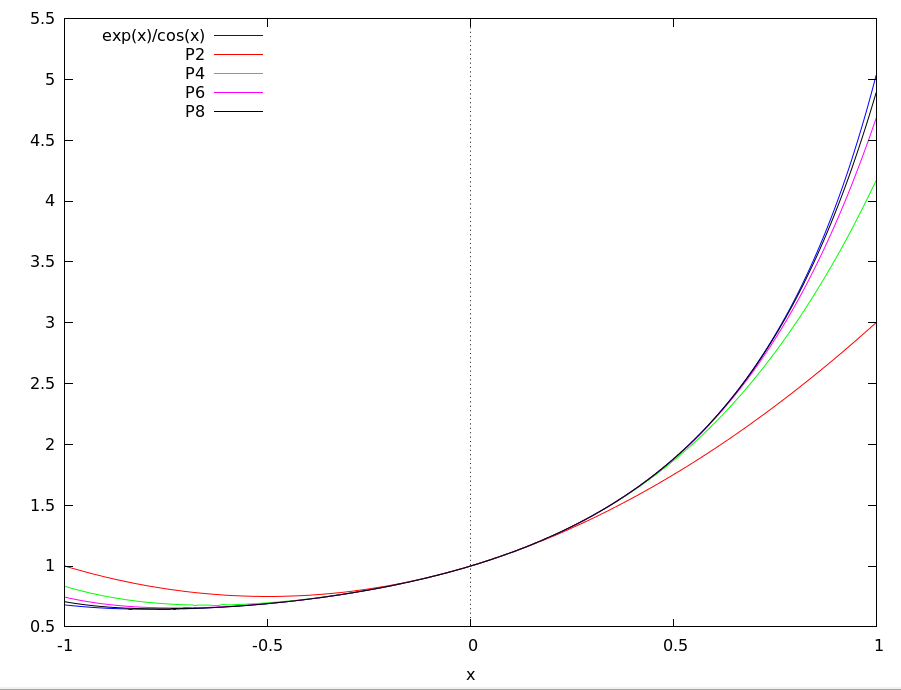
\includegraphics[width=10cm]{exp_cos.png}
\end{figure}

\section{Función (1+x)exp(x)}
Ejemplificar la aproximación de Taylor de la función (1+x) exp(x), alrededor de x=0.

\subsection{Código en Maxima}

 \begin{verbatim}
f(x):= (1+x)*exp(x);
T3(x):=taylor(f(x), x, 0, 3);
T9(x):=taylor(f(x), x, 0, 9);
T13(x):=taylor(f(x), x, 0, 13);
T15(x):=taylor(f(x), x, 0, 15);
fortran(T3(x));
fortran(T9(x));
fortran(T13(x));
fortran(T15(x));
tex(T3(x));
tex(T9(x));
tex(T13(x));
tex(T15(x));
plot2d ([f(x),T3(x), T9(x), T13(x), T15(x)], [x, -6, 2], [y, -2, 6],
[legend, "(1+x)exp(x)", "P3", "P9", "P13","P15"],
[gnuplot_preamble, "set key left"],
[color, blue, green, orange,red,violet],[box,false]);
\end{verbatim}

\subsection{Gráfica}

\begin{figure}[h]
\centering
\includegraphics[width=10cm]{_1+x_expx.png}
\end{figure}

\section{Conclusión}
En conclusión, gnuplot es una herramienta muy útil a la hora de realizar gráficas ,ya que cuenta con muchas opciones para graficar o modificar las gráficas. Al principio puede parecer un tanto complicada de usar, pero el saber usarla puede llegar a facilitar muchas tareas.





\end{document}
